\section{Durchführung und Aufbau}
\label{sec:Durchführung}
In einen evakuierten Glaszylinder kann ein $\text{Americium}^{241}$ Präperat auf einer Schiene zum Sperrschichtzähler verschoben werden. Es wird ein Sperrschichtzähler gewählt, weil dieser bereits bei geringeren Energien Ionisierend Strahlung wahrnimmt. Über einen Kompressor kann der Druck im Zylinder variiert werden. Mittels einer Diskreminatorschwelle wird versucht die Hintergrundstrahlung gering zu halten. Ein Schematischer Aufbau ist in Abbildung \ref{fig:Auf} zu sehe.
\begin{figure}
  \centering
  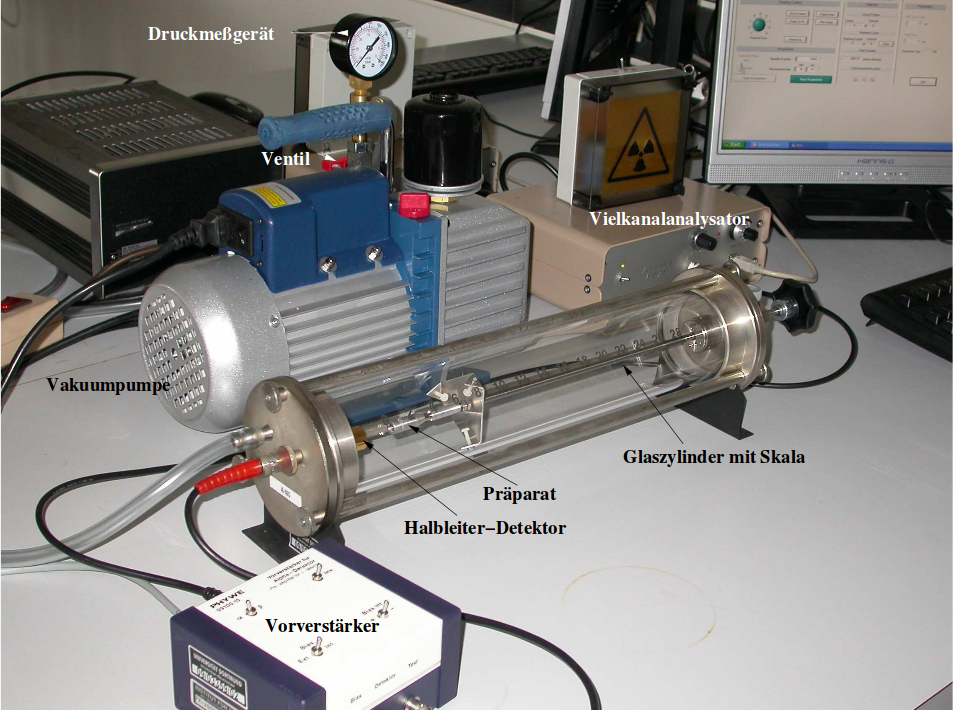
\includegraphics[height=6cm]{Aufbau.png}
  \caption{Versuchsaufbau}
  \label{fig:Auf}
\end{figure}
Mittels eines Vielkanalanalysator werden die Messungen über eine PC ausgewertet. Zunächst wird bei einem konstanteten Abstand der Druck variiert und die gemessenen Pulse, sowie der am Häufigst auftretene Channel für 20 verschiedene Drücke entnommen. Ein höherer Channel entspricht einer größreren Energie des Teilchens. 
Desweiteren sollen Hundert Werte für eine Statistik aufgenommen und in einem Histogrammm dargestellt werden. Dieses soll einerseits mit der Poisson- als auch mit der Gaußverteilung verglichen werden. 
